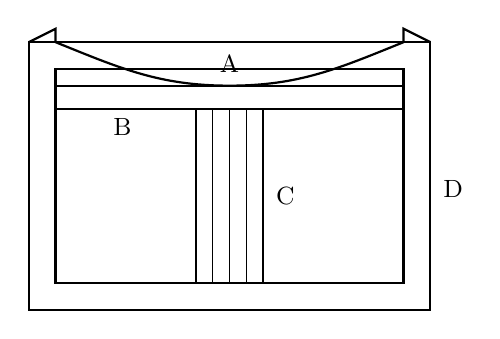
\begin{tikzpicture}[scale=0.85,font=\small]
  % Outer frame D
  \draw[thick] (0, 0) rectangle (6.0, 4.0);
  \draw[thick] (0.4, 0.4) rectangle (5.6, 3.6);
  % Small corner notches at top
  \draw[thick] (0, 4.0) -- (0.4, 4.2) -- (0.4, 4.0);
  \draw[thick] (6.0, 4.0) -- (5.6, 4.2) -- (5.6, 4.0);
  \node[right] at (6.05, 1.8) {D};

  % Plano-convex lens A fixed at top inner edge
  \draw[thick] (0.4, 4.0) -- (5.6, 4.0);
  \draw[thick] (0.4, 4.0) to[out=-22,in=180] (3.0, 3.35) to[out=0,in=-158] (5.6, 4.0);
  \node at (3.0, 3.68) {A};

  % Flat glass plate B resting on metal column C
  \draw[thick] (0.4, 3.0) rectangle (5.6, 3.35);
  \node[below] at (1.4, 3.0) {B};

  % Metal column C (vertical rod/cylinder with shading lines)
  \draw[thick] (2.5, 0.4) rectangle (3.5, 3.0);
  \draw[thin] (2.75, 0.4) -- (2.75, 3.0);
  \draw[thin] (3.0, 0.4) -- (3.0, 3.0);
  \draw[thin] (3.25, 0.4) -- (3.25, 3.0);
  \node[right] at (3.55, 1.7) {C};
\end{tikzpicture}
